\documentclass{beamer}

\usepackage{amsmath,cancel}
\usepackage{graphicx}
\usepackage{color}
\usepackage{alltt}

\newcommand{\sect}[1]{
\section{#1}
\begin{frame}[fragile]\frametitle{#1}
}

\newcommand{\bi}{\begin{itemize}}
\newcommand{\ii}{\item}
\newcommand{\ei}{\end{itemize}}

\begin{document}
\sect{Using trees to guess}
\bi
\ii  Find a good guess for
\begin{align*}
  T(n) &= 3T(n/4) + \Theta(n^2)
\end{align*}
\ei

\end{frame}
\sect{}
\includegraphics[height=0.9\textheight]{Fig-4-5.pdf}
\end{frame}

\sect{Bound the summation}
\small
\bi
\ii
A geometric series of a number less than 1 can be bounded:
\begin{align*}
  T(n) &= cn^2 + \frac{3}{16}cn^2 + \left(\frac{3}{16}\right)^2cn^2 + ...
  + \left(\frac{3}{16}\right)^{\log_4 n - 1}cn^2 + \Theta(n^{\log_4 3})\\
  &= \sum_{i=0}^{\log_4n - 1} \left(\frac{3}{16}\right)^icn^2
  + \Theta(n^{\log_4 3})\\
  &< \sum_{i=0}^{\infty} \left(\frac{3}{16}\right)^icn^2
  + \Theta(n^{\log_4 3})\\
  &= \frac{1}{1-(3/16)}cn^2  + \Theta(n^{\log_4 3})\\
  &= \frac{16}{13}cn^2  + \Theta(n^{\log_4 3})\\
  &= O(n^2)
\end{align*}
\ii
Now we can check this guess with substitution (induction).
\ei
\end{frame}


\sect{Explicitly Solving Recursion of p. 89}
\begin{eqnarray*}
T(n) &=& \cancel{3T\left(\frac{n}{4}\right)}+ cn^2\\
\cancel{3T\left(\frac{n}{4}\right)} &=& \cancel{3^2T\left(\frac{n}{4^2}\right) } + 3c\left(\frac{n}{4}\right)^2\\
\cancel{3^2T\left(\frac{n}{4^2}\right)} &=& \cancel{3^3T\left(\frac{n}{4^3}\right)}  + 3^2c\left(\frac{n}{4^2}\right)^2\\
\cancel{3^3T\left(\frac{n}{4^3}\right)} &=& \cancel{3^4T\left(\frac{n}{4^4}\right)}  + 3^3c\left(\frac{n}{4^3}\right)^2\\
&...&\\
\cancel{3^{k-1}T\left(\frac{n}{4^{k-1}}\right)} &=& \cancel{3^{k}T\left(\frac{n}{4^{k}}\right)}  + 3^{k-1}c\left(\frac{n}{4^{k-1}}\right)^2\\
&...&\\
\cancel{3^{\log_4 n-1}T\left(\frac{n}{4^{\log_4 n-1}}\right)} &=& 3^{\log_4 n}T\left(\frac{n}{4^{\log_4 n}}\right)  + 3^{\log_4 n-1}c\left(\frac{n}{4^{\log_4 n-1}}\right)^2\\
T(n) &=&3^{\log_4 n}T\left(\frac{n}{4^{\log_4 n}}\right)  + \sum_{i=0}^{\log_4 n-1}3^{i}c\left(\frac{n}{4^{i}}\right)^2\\
\end{eqnarray*}
\end{frame}

\sect{Explicitly Solving Recursion of p. 89}
\begin{align*}
  T(n) &=
  3^{\log_4 n}T\left(\frac{n}{4^{\log_4 n}}\right)
  + \sum_{i=0}^{\log_4 n-1}3^{i}c\left(\frac{n}{4^{i}}\right)^2\\
  &=   n^{\log_4 3}T(1)
  + cn^2\sum_{i=0}^{\log_4 n-1}\left(\frac{3}{16}\right)^i\\
  &=
     n^{\log_4 3}T(1)
     + cn^2\left(\frac{(3/16)^{\log_4 n} - 1}{(3/16)-1}\right)\\
 &= \Theta(n^2)
     \end{align*}


\end{frame}


\sect{Second recursion tree example}
\footnotesize
\[ T(n) = T(n/3) + T(2n/3) + O(n) \]
\vfill

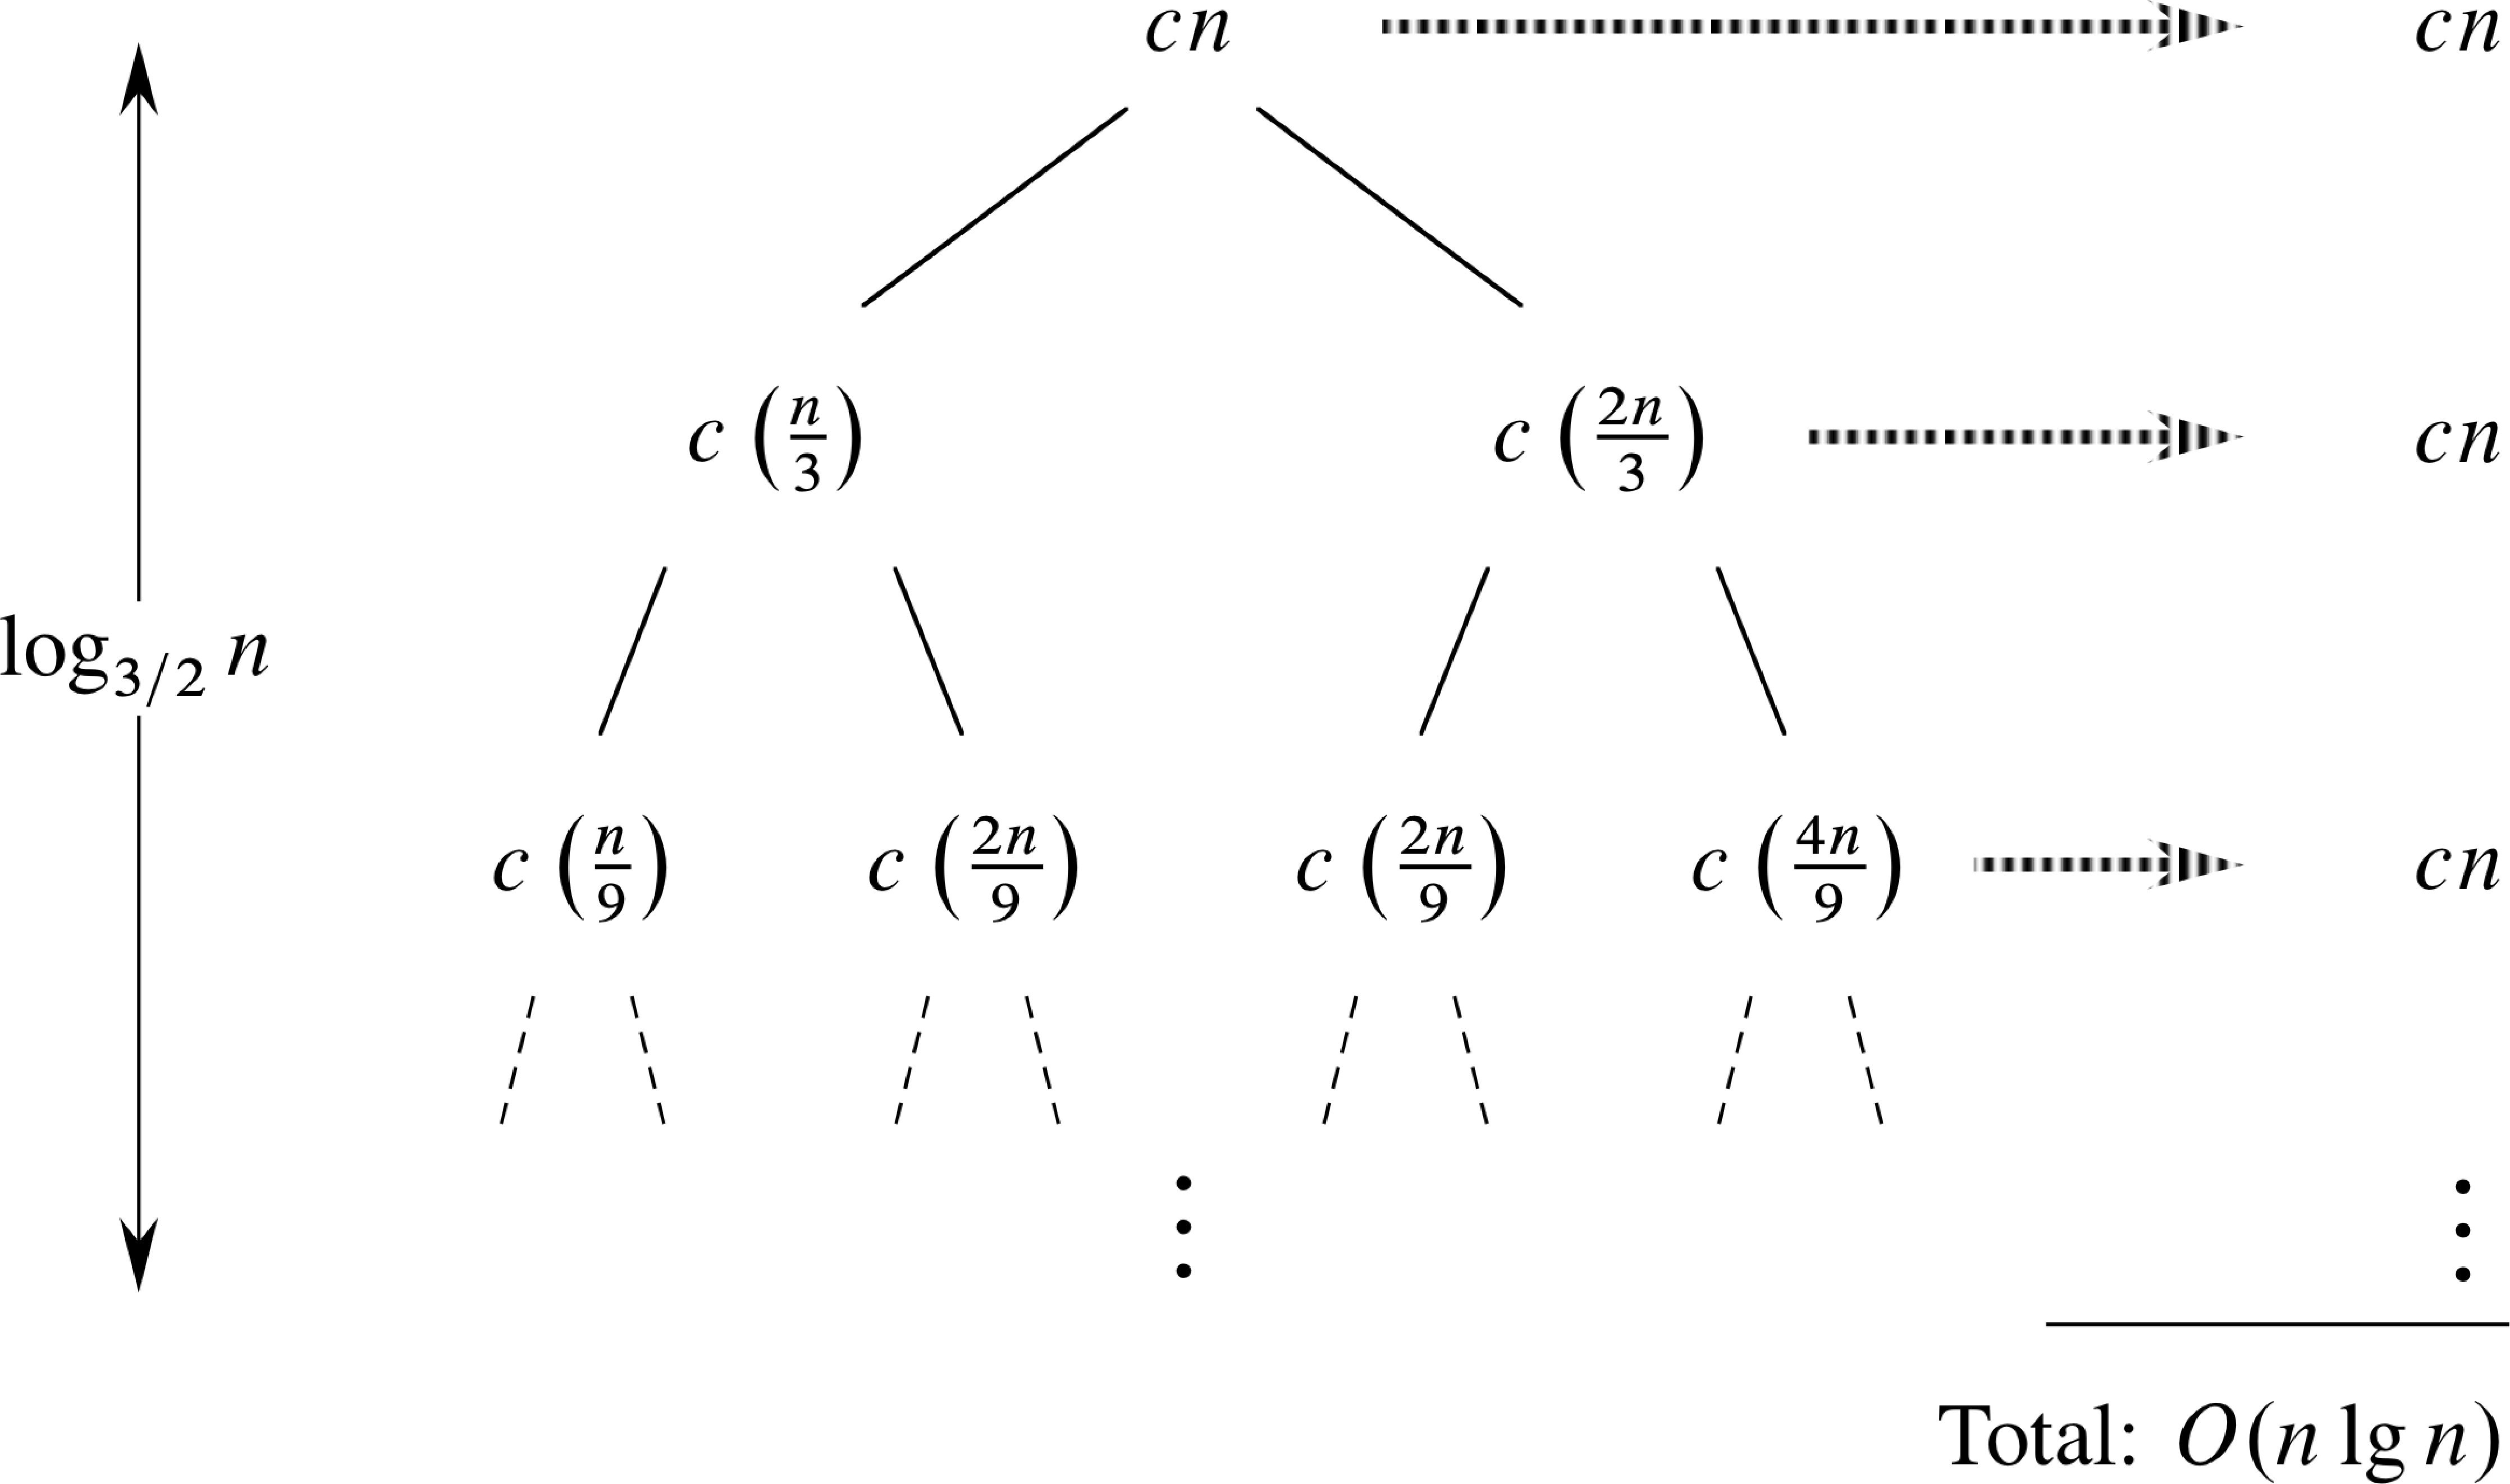
\includegraphics[scale=0.1]{Fig-4-6.pdf}
\bi
\pause
\ii Prove your guess with substitution (induction).
\pause
\ii Can you bound the leaves?
\pause
\ii $n^{\log_{3/2} 2} \approx n^{1.7} =\Omega(n\lg n)$
\pause
\ii Substitution will assure you this is not a problem.
\ei

\end{frame}


\end{document}





